\begin{center}

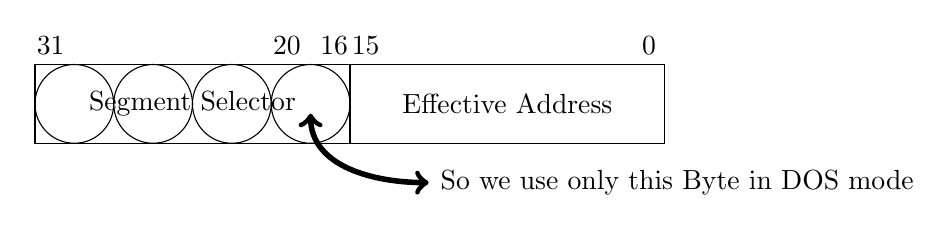
\begin{tikzpicture}
\coordinate [label=above:31] (A) at (0.2,1);
\coordinate [label=above:20] (A) at (3.2,1);
\coordinate [label=above:16] (A) at (3.8,1);
\coordinate [label=above:15] (A) at (4.2,1);
\coordinate [label=above:0] (A) at (7.8,1);
\draw (0,0) rectangle (4,1) node[pos=.5] {Segment Selector};
\draw (4,0) rectangle (8,1) node[pos=.5] {Effective Address};
\foreach \x in {1,2,3,4}
	\draw[baseline] (\x-0.5,0.5 ) node (N\x) {} circle (0.5);
\draw[<->,line width =2pt] [out=-90] (N4)  to [in=180] (5,-0.5) node[right]{So we use only this Byte in DOS mode} ;
\end{tikzpicture}
	
\end{center}